
\chapter{Design}

In the design section, we will detail the process of translating Ataccama's expression language into Python, focusing on local execution and user-friendliness. The aim is to allow data engineers to seamlessly integrate Ataccama's data quality rules into their Python workflows. This section outlines the architecture, methodologies, and tools necessary to adapt Ataccama expressions for effective use in Python environments, ensuring the solution is both practical and easy to use.

\section{Context of data transformations}

Data processing pipelines typically adhere to a structured pattern known as \glsxtrfull{etl}\cite{etl}\ref{fig:etl_process}, crucial in data management. These pipelines start by extracting data from various sources, which is then transformed through cleaning, enrichment, and aggregation processes before being loaded into a final storage destination.

This thesis specifically concentrates on this transformation step, where data quality rules can be effectively implemented and integrated.

\begin{figure}[ht]
    \centering
    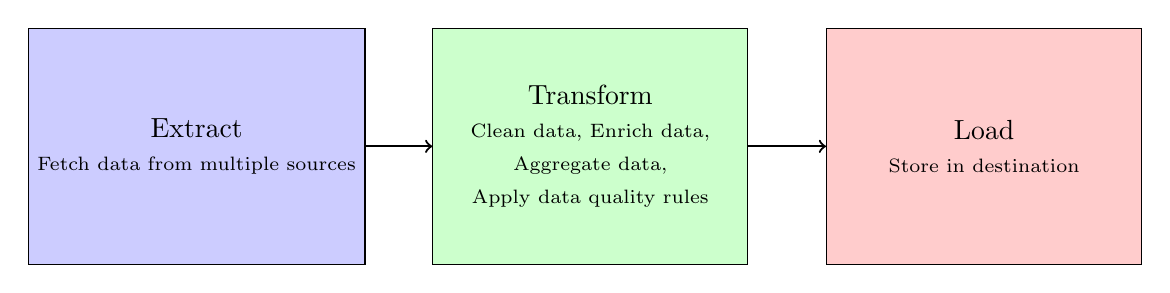
\begin{tikzpicture}
        % Draw boxes
        \node[draw, rectangle, align=center, minimum height=3cm, minimum width=4cm, fill=blue!20] (extract) at (0,0) {Extract \\ \scriptsize Fetch data from multiple sources};
        \node[draw, rectangle, align=center, minimum height=3cm, minimum width=4cm, fill=green!20] (transform) at (5,0) {Transform \\ \scriptsize Clean data, Enrich data, \\ \scriptsize Aggregate data, \\ \scriptsize Apply data quality rules};
        \node[draw, rectangle, align=center, minimum height=3cm, minimum width=4cm, fill=red!20] (load) at (10,0) {Load \\ \scriptsize Store in destination};
    
        % Draw arrows
        \draw[->, thick] (extract.east) -- (transform.west);
        \draw[->, thick] (transform.east) -- (load.west);
    \end{tikzpicture}
    \caption{Diagram illustrating the \glsxtrfull{etl} process.}
    \label{fig:etl_process}
    \end{figure}

\section{Interface design}

The design of the API is straightforward due to the simplicity of the public functionality it offers. Below is a diagram that outlines the public interface of the transpiler:

\begin{figure}[htbp]
    \centering
    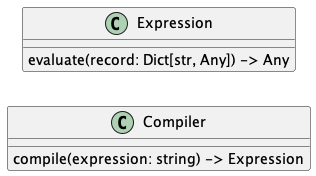
\includegraphics[scale=0.7]{diagrams/api_design-class.png}
    \caption{API overview}
    \label{fig:api}
\end{figure}

The interface is uncomplicated, designed primarily to compile and execute expressions efficiently. This simplicity ensures that all essential actions—compiling an expression and executing it—are both intuitive and accessible for users.

The API consists of two primary classes: \texttt{Compiler} and \texttt{Expression}. The \texttt{Compiler} class is responsible for compiling the expression into Python code, while the \texttt{Expression} class encapsulates the compiled code and provides a method to execute it with a given record. The record is supplied as a dictionary, where the keys correspond to the field names and the values to the field values.

\section{Architecture}

The initial step in developing the solution involves establishing its architecture, which is critical for defining how the program will function. 

The architecture of the Python implementation of the Ataccama Expression Language is designed to facilitate the translation of Ataccama's expression language into Python code to enable for local execution, one of the goals of outlined in analysis. This translation process involves parsing the input expression, generating executable code, and evaluating the expression against a dataset. The architecture is structured to accommodate these steps seamlessly, ensuring the efficient execution of data quality rules within a Python environment.

For the first step, the input expression will be converted into an abstract syntax tree (AST). Given the complexity of the expression language used by Ataccama, employing a parser generator is deemed the most effective approach. The parser generator will utilize the predefined grammar of the language to generate a parser capable of translating input expressions into an AST. This facilitates the incorporation of custom logic in the subsequent steps, particularly during the semantic analysis phase.

During semantic analysis, the AST will be traversed to construct executable code. This transformation is essential for preparing the expression for evaluation in a Python environment, from which the results can be dynamically generated and returned.

The final component of the architecture involves executing the generated code on the provided records. This step ensures that each record is evaluated according to the defined expressions, and the outcomes are systematically returned to the user.

\subsection{Parser generator}

For the parser generator, a specific approach is indicated. The Ataccama Expression Language implementation uses a parser generator called ANTLR. ANTLR (ANother Tool for Language Recognition) is a powerful parser generator\cite{antlr}. It's widely used to build languages, tools, and frameworks. From a grammar, ANTLR generates a parser that can build and walk parse trees\cite{antlr4docs}. As the grammar of the Ataccama Expression Language is already defined, it is simple and robust to use, adapt and reuse the grammar by also using ANTLR to generate the parser. 

\subsection{Code generation}

Having decided on the parser generator, the next step is to decide how to generate the code for the expression. There are two obvious approaches at hand: Represent the expression in an object tree with execution being a recursive descent through the tree. The second approach is to generate Python code directly. This can be done using Python standard module \texttt{ast}, which can be used build an abstract syntax tree of the expression, and then compile it into a Python function. Alternatively, the code can be generated as a string and then executed using Python's exec function, but this approach is less safe, more error-prone, harder to debug and introduces more overhead as it adds an additional step of parsing the code.

The second approach is more efficient, as it avoids the overhead of traversing the AST, but it is also more complex, as it requires generating Python code. The first approach might appear simpler, but it is less efficient, as it requires traversing the AST and does not include the option to use compilation to Python bytecode.

Using Python as the runtime also comes with the benefit of being able to use Python's scope resolution and name hiding to implement the scoping rules of the Ataccama Expression Language, so a reimplementation can be avoided.

For these reasons, the second approach is chosen. The code will be generated as Python code using the ast module, and then compiled into a Python module.

\section{Compatibility with the Ataccama Expression language}

The Ataccama Expression Language is complex and has many features, along with
platform specific quirks a peculiarities. For this reason, the implementation will
not be a one-to-one copy of the language, but rather a subset of the language
features that are most commonly used with some differences in behaviour.

The differences between the Ataccama Expression Language and the Python
implementation will be outlined in detail in the following sections. As the goal
is to make the implementation as close to the original language as possible, the
differences will be kept to a minimum. Consequently, the implementation will be
able to run most of the data quality rules written in the Ataccama Expression
Language.

To ensure compatibility, the test suite will be created based on the Ataccama Expression Language test suite. The test suite will be used to validate the implementation and ensure that it behaves as expected.

The rest of this section describes a high-level overview of the differences that
will have to be introduced along with the reasons behind them. Most of the
differences are a result of a different underlying technology, decisions have to be
made on where to draw the line between mimicking the original language and

This section has two purposes: The first is to describe the language and its features, the second is to outline and discuss design decisions related to the individual fetatures and functionality that have to be made in order to implement the language in Python 
introducing accepting differences for the sake of simplicity and performance.

\subsection{Dynamic typing}

The Ataccama Expression Language is statically typed, following its language
of implementation which is Java. This means that the type of each variable and
expression is known at compile time compile time. This allows the compiler to
catch type errors at compile time, and to generate more efficient code. Also,
it allows for function and operator overloading, as the compiler can choose the
correct function based on the types of the arguments.
This is possible thanks to the record format being known at compile time. The
record format is a schema that defines the types of the fields in the record.
Python is dynamically typed, which means that it is possible to allow for
dynamic typing in the implementation.

On the other hand, to reimplement static typing in Python would require
aditional work like keeping track of the types of all symbols and expressions and
resolving function overloads.

Furthermore, static typing would require the user to define the record format
at compile time, which would make the API less user-friendly, which in our case
is a priority. This could be solved by allowing the user to define the record format optionally.

Considering the above stated arguments, the decision is to allow for dynamic
typing in the implementation, as it is easier to implement and more flexible. 
The implementation of optional static typing is a possible future improvement, but for the initial implementation would
constitute a great effort for little gain from the user's perspective.

\subsubsection{Function and operator overloading}

The decision to utilize dynamic typing in the Python implementation of the Ataccama Expression Language carries significant implications for function and operator overloading. Unlike in Java, where Ataccama's static typing enables the compiler to select the correct function or operator based on argument types at compile time, Python's dynamic typing means the types of variables are only known at runtime. This characteristic prevents overloading functions and operators based on type, as there is no way to determine the type of the inputs beforehand.

As a result, each function in the Python implementation must be universally applicable, handling all expected input types through internal logic. This requires implementing comprehensive type checking within each function, where the function determines the appropriate action based on the runtime types of the arguments. Such an approach aligns with Python’s duck typing philosophy, where operations are attempted regardless of type, with the function internally managing any type mismatches or errors. This method ensures flexibility and broad applicability of functions, albeit at the cost of the type-specific optimization possible in statically typed languages like Java.

\subsection{Implementation scope}

The Ataccama Expression Language supports over 150 functions but the implementation in Python will be limited to a subset of
the language features. The reasoning behind this is that many of the functions are
not commonly used, and the implementation of all of them would be a significant
effort and would be out of scope for this project as the goal is to provide a simple
prototype and validate the viability first. 

For this reason, the functions have been categorized by priority, and the implementation will
focus on the high- and medium-priority functions. The categorization is based on the frequency of use of the tasks in the data quality rules, and the complexity of the implementation. The high-priority functions are the most commonly used functions, and the medium-priority functions are less commonly used but still important. 
The prioritization comes from Ataccama's knowledge base. The low-priority functions are the least commonly used functions, and will not be implemented in the initial version of the implementation. 

A list of all function along with their priority and implementation status can be found in the appendix \ref{app:list-of-functions}.


\subsection{Arithmetic}
The Ataccama Expression Language operates, like standard types in Java, in
fixed-size bit arithmetic, i.e., 32 bits for integers and 64 bits for Python. 
On the other hand, Python uses arbitrary precision arithmetic, which means that the size
of the integers is not limited. This means that the results of arithmetic operations
can differ between the two languages.
For everyday operations, the difference is not significant, and it could be said
that the Python behaviour is better. However, in some use cases, the fixed-size
arithmetic is necessary, for example, when working with hash tables. As the number
of these cases is limited and most of them are provided as implemented functionality,
the implementation will use Python-native arbitrary precision arithmetic and
handle fixed-size arithmetic as a special case where necessary.

Furthermore, the Ataccama Expression Language provides arithmetic operators
for addition, subtraction, multiplication, division, integer division, and remainder. 
Python provides the same operators, but
the behaviour of the operators is different. The first significant difference
is the handling of null values. In Ataccama Expression Language, the operators are null safe and
follow a SQL-like behaviour. In Python, the operators throw an exception if any of the operands is null.
Also, the arithmetics are different; modulo and division produce different results for negative operands. These differences will have to be addressed as the
results differ too much to be ignored.  Moreover, Python uses arbitrary precision arithmetic, whereas Ataccama Expressions use the underlying Java types, but this difference is not significant for most use cases and could be considered an improvement. 
Lastly, the plus operator in Ataccama Expression Language is overloaded for string concatenation, converting any non-string to string first, which is not the case in Python. This will have to be implemented as it is a common use case.


\subsection{Null handling and null coalescing}

The way Ataccama Expression language handles nulls has a lot of aspects
which have to be addressed.

Operators handle null values in a SQL-like way, mostly returning null if any
of the operands is null. The implication for the implementation is that it will not be
possible to use native Python operators, as they do not handle null values in the
same way.

Empty strings are treated as null values. The documentation states: "A null
string and an empty string are considered equal". Moreover, in the Ataccama Expression Language, most empty string
returns are coalesced to null. This behaviour also has its own quirks, for example
‘1 + null == null‘ but ‘1 + "" == "1"‘, which breaks the aforementioned statement.

Furthermore, functions have to be prepared to handle null values in any of the
arguments. Most commonly, functions return null if any of the arguments is null,
so extensive null checking has to be implemented in the functions.
The implementation in Python will have to address these differences and
provide a way to handle null values in a Python environment.
Date and floating point formatting

\section{Summary}

The design of the Python implementation of the Ataccama Expression Language is structured to facilitate the translation of Ataccama's expression language into Python code for local execution. The architecture is designed to accommodate the parsing of input expressions, the generation of executable code, and the evaluation of expressions against a dataset. The implementation will focus on a subset of the language features, prioritizing high- and medium-priority functions based on their frequency of use and complexity. The implementation will also address key differences between the Ataccama Expression Language and Python, such as dynamic typing, null handling, and arithmetic operations, to ensure compatibility and functionality. The design decisions outlined in this section provide a roadmap for the development of the Python implementation, guiding the translation of the Ataccama Expression Language into a Python environment for accessible and easy data quality rule execution.